\documentclass{whiteboard}
\begin{document}
\begin{frame}[plain,t]
 \bbcover{Educational Codeforces Round 33}{Problem C -- Rumor}{Prof. Edson Alves}{Faculdade UnB Gama}
\end{frame}

\begin{frame}[plain,t]
\vspace*{\fill}
 \bbenglish{Vova promised himself that he would never play computer games... But recently Firestorm -- a well-known game developing company -- published their newest game, World of Farcraft, and it became really popular. Of course, Vova started playing it.}

 \vspace{0.2in}

 \bbenglish{Now he tries to solve a quest. The task is to come to a settlement named Overcity and spread a rumor in it.}

 \vspace{0.2in}

 \bbenglish{Vova knows that there are $n$ characters in Overcity. Some characters are friends to each other, and they share information they got. Also Vova knows that he can bribe each character so he or she starts spreading the rumor; $i$-th character wants $c_i$ gold in exchange for spreading the rumor. When a character hears the rumor, he tells it to all his friends, and they start spreading the rumor to their friends (for free), and so on.}
\vspace*{\fill}
\end{frame}

\begin{frame}[plain,t]
\vspace*{\fill}
 \bbtext{Vova prometeu a si mesmo que ele nunca jogaria jogos de computador... Mas recentemente Firestorm -- uma companhia de desenvolvimento de jogos bem conhecida -- publicou seu jogo mais recente, World of Farcraft, e ele se tornou realmente popular. Evidentemente, Vova começou a jogá-lo.}

 \vspace{0.2in}

 \bbtext{Agora ele está tentando finalizar uma missão. A tarefa é ir a um assentamento chamado Overcity e espalhar um rumor nele.}

 \vspace{0.2in}

 \bbtext{Vova sabe que há $n$ personagens em Overcity. Algumas personagens são amigas umas das outras, e elas compartilham as informações que obtém. Vova também sabe que ele pode subornar uma personagem de modo que ele ou ela inicie o rumor; a $i$-ésima personagem quer $c_i$ moedas de ouro para espalhar o rumor. Quando uma personagem ouve um rumor, ela o espalha a todos seus amigos, e estes repassam o rumor a seus amigos (de graça), e assim por diante.}
\vspace*{\fill}
\end{frame}

\begin{frame}[plain,t]
\vspace*{\fill}
 \bbenglish{The quest is finished when all $n$ characters know the rumor. What is the minimum amount of gold Vova needs to spend in order to finish the quest?}

 \vspace{0.2in}

 \bbenglish{Take a look at the notes if you think you haven't understood the problem completely.}
\vspace*{\fill}
\end{frame}

\begin{frame}[plain,t]
\vspace*{\fill}
 \bbtext{A missão termina quando todas $n$ personagens tem conhecimento do rumor. Qual é a menor quantidade de moedas de ouro que Vova precisa gastar para finalizar a missão?}

 \vspace{0.2in}

 \bbtext{Observe as notas se você não tenha entendido o problema completamente.}
\vspace*{\fill}
\end{frame}

\begin{frame}[plain,t]
\vspace*{\fill}
 \bbbold{Input}

 \vspace{0.1in}

 \bbenglish{The first line contains two integer numbers $n$ and $m$ $(1\leq n\leq 10^5, 0\leq m\leq 10^5)$ -- the number of characters in Overcity and the number of pairs of friends.}

 \vspace{0.1in}

 \bbenglish{The second line contains $n$ integer numbers $c_i$ $(0\leq c_i\leq 10^9)$ -- the amount of gold $i$-th character asks to start spreading the rumor.}

 \vspace{0.1in}

 \bbenglish{Then $m$ lines follow, each containing a pair of numbers $(x_i, y_i)$ which represent that characters $x_i$ and $y_i$ are friends $(1\leq x_i, y_i\leq n, x_i\neq y_i)$. It is guaranteed that each pair is listed at most once.}

 \vspace{0.2in}

 \bbbold{Output}

 \vspace{0.1in}

 \bbenglish{Print one number -- the minimum amount of gold Vova has to spend in order to finish the quest.}
\vspace*{\fill}
\end{frame}

\begin{frame}[plain,t]
\vspace*{\fill}
 \bbbold{Entrada}

 \vspace{0.1in}

 \bbtext{A primeira linha contém dois inteiros $n$ e $m$ $(1\leq n\leq 10^5, 0\leq m\leq 10^5)$ -- o número de personagens em Overcity e o número de pares de amigos.}

 \vspace{0.1in}

 \bbtext{A segunda linha contém $n$ números inteiros $c_i$ $(0\leq c_i\leq 10^9)$ -- a quantidade de moedas de ouro que a $i$-ésima personagem quer para começar a espalhar o rumor.}

 \vspace{0.1in}

 \bbtext{As $m$ linhas seguintes contém, cada uma, um par de números $(x_i, y_i)$ que indicam que as personagens $x_i$ e $y_i$ são amigas $(1\leq x_i, y_i\leq n, x_i\neq y_i)$. É garantido que cada par é listado, no máximo, uma vez.}

 \vspace{0.2in}

 \bbbold{Output}

 \vspace{0.1in}

 \bbtext{Imprima um número -- a quantidade mínima de moedas de ouro que Vova tem que gastar para completar a missão.}
\vspace*{\fill}
\end{frame}

\begin{frame}[plain,t]
\begin{tikzpicture}
\node[draw,opacity=0] at (0, 0) {x};
\node[draw,opacity=0] at (14, 8) {x};
 \node[anchor=west] at (0, 7) { \bbbold{Exemplo de entrada e saída} };
\end{tikzpicture}
\end{frame}

\begin{frame}[plain,t]
\begin{tikzpicture}
\node[draw,opacity=0] at (0, 0) {x};
\node[draw,opacity=0] at (14, 8) {x};
 \node[anchor=west] at (0, 7) { \bbbold{Exemplo de entrada e saída} };
 \node[anchor=west] at (1, 6) { \bbtext{5 2} };
\end{tikzpicture}
\end{frame}

\begin{frame}[plain,t]
\begin{tikzpicture}
\node[draw,opacity=0] at (0, 0) {x};
\node[draw,opacity=0] at (14, 8) {x};
 \node[anchor=west] at (0, 7) { \bbbold{Exemplo de entrada e saída} };
 \node[anchor=west] at (1, 6) { \bbtext{5 2} };
 \node at (1.2, 5) { \footnotesize \bbcomment{\# de personagens} };
 \draw[->,color=BBViolet] (1.2, 5.2) -- (1.2, 5.8);
\end{tikzpicture}
\end{frame}

\begin{frame}[plain,t]
\begin{tikzpicture}
\node[draw,opacity=0] at (0, 0) {x};
\node[draw,opacity=0] at (14, 8) {x};
 \node[anchor=west] at (0, 7) { \bbbold{Exemplo de entrada e saída} };
 \node[anchor=west] at (1, 6) { \bbtext{5 2} };
 \node at (1.2, 5) { \footnotesize \bbcomment{\# de personagens} };
 \draw[->,color=BBViolet] (1.2, 5.2) -- (1.2, 5.8);
 \node[anchor=west] at (2.6, 6) { \footnotesize \bbcomment{\# de pares de amigos} };
 \draw[->,color=BBViolet] (1.8, 6) -- (2.5, 6);
\end{tikzpicture}
\end{frame}

\begin{frame}[plain,t]
\begin{tikzpicture}
\node[draw,opacity=0] at (0, 0) {x};
\node[draw,opacity=0] at (14, 8) {x};
 \node[anchor=west] at (0, 7) { \bbbold{Exemplo de entrada e saída} };
 \node[anchor=west] at (1, 6) { \bbtext{5 2} };
 \node[anchor=west] at (1, 5) { \bbtext{2 5 3 4 8} };
\end{tikzpicture}
\end{frame}

\begin{frame}[plain,t]
\begin{tikzpicture}
\node[draw,opacity=0] at (0, 0) {x};
\node[draw,opacity=0] at (14, 8) {x};
 \node[anchor=west] at (0, 7) { \bbbold{Exemplo de entrada e saída} };
 \node[anchor=west] at (1, 6) { \bbtext{5 2} };
 \node[anchor=west] at (1, 5) { \bbtext{2 5 3 4 8} };
 \node[anchor=west] at (4.2, 5) { \footnotesize \bbcomment{custo individual para iniciar o rumor} };
 \draw[->,color=BBViolet] (3.2, 5) -- (4.1, 5);
\end{tikzpicture}
\end{frame}

\begin{frame}[plain,t]
\begin{tikzpicture}
\node[draw,opacity=0] at (0, 0) {x};
\node[draw,opacity=0] at (14, 8) {x};
 \node[anchor=west] at (0, 7) { \bbbold{Exemplo de entrada e saída} };
 \node[anchor=west] at (1, 6) { \bbtext{5 2} };
 \node[anchor=west] at (1, 5) { \bbtext{2 5 3 4 8} };
 \node[draw,circle,very thick] (A) at (6, 4) { \bbtext{1}$^{\bbcomment{2}}$ };
 \node[draw,circle,very thick] (B) at (9, 7) { \bbtext{2}$^{\bbcomment{5}}$ };
 \node[draw,circle,very thick] (C) at (12, 6) { \bbtext{3}$^{\bbcomment{3}}$ };
 \node[draw,circle,very thick] (D) at (12, 2) { \bbtext{4}$^{\bbcomment{4}}$ };
 \node[draw,circle,very thick] (E) at (9, 1) { \bbtext{5}$^{\bbcomment{8}}$ };
\end{tikzpicture}
\end{frame}

\begin{frame}[plain,t]
\begin{tikzpicture}
\node[draw,opacity=0] at (0, 0) {x};
\node[draw,opacity=0] at (14, 8) {x};
 \node[anchor=west] at (0, 7) { \bbbold{Exemplo de entrada e saída} };
 \node[anchor=west] at (1, 6) { \bbtext{5 2} };
 \node[anchor=west] at (1, 5) { \bbtext{2 5 3 4 8} };
 \node[draw,circle,very thick] (A) at (6, 4) { \bbtext{1}$^{\bbcomment{2}}$ };
 \node[draw,circle,very thick] (B) at (9, 7) { \bbtext{2}$^{\bbcomment{5}}$ };
 \node[draw,circle,very thick] (C) at (12, 6) { \bbtext{3}$^{\bbcomment{3}}$ };
 \node[draw,circle,very thick] (D) at (12, 2) { \bbtext{4}$^{\bbcomment{4}}$ };
 \node[draw,circle,very thick] (E) at (9, 1) { \bbtext{5}$^{\bbcomment{8}}$ };
 \node[anchor=west] at (1, 4) { \bbtext{1 4} };
\end{tikzpicture}
\end{frame}

\begin{frame}[plain,t]
\begin{tikzpicture}
\node[draw,opacity=0] at (0, 0) {x};
\node[draw,opacity=0] at (14, 8) {x};
 \node[anchor=west] at (0, 7) { \bbbold{Exemplo de entrada e saída} };
 \node[anchor=west] at (1, 6) { \bbtext{5 2} };
 \node[anchor=west] at (1, 5) { \bbtext{2 5 3 4 8} };
 \node[draw,circle,very thick] (A) at (6, 4) { \bbtext{1}$^{\bbcomment{2}}$ };
 \node[draw,circle,very thick] (B) at (9, 7) { \bbtext{2}$^{\bbcomment{5}}$ };
 \node[draw,circle,very thick] (C) at (12, 6) { \bbtext{3}$^{\bbcomment{3}}$ };
 \node[draw,circle,very thick] (D) at (12, 2) { \bbtext{4}$^{\bbcomment{4}}$ };
 \node[draw,circle,very thick] (E) at (9, 1) { \bbtext{5}$^{\bbcomment{8}}$ };
 \node[anchor=west] at (1, 4) { \bbtext{1 4} };
 \draw[thick] (A) to (D);
\end{tikzpicture}
\end{frame}

\begin{frame}[plain,t]
\begin{tikzpicture}
\node[draw,opacity=0] at (0, 0) {x};
\node[draw,opacity=0] at (14, 8) {x};
 \node[anchor=west] at (0, 7) { \bbbold{Exemplo de entrada e saída} };
 \node[anchor=west] at (1, 6) { \bbtext{5 2} };
 \node[anchor=west] at (1, 5) { \bbtext{2 5 3 4 8} };
 \node[draw,circle,very thick] (A) at (6, 4) { \bbtext{1}$^{\bbcomment{2}}$ };
 \node[draw,circle,very thick] (B) at (9, 7) { \bbtext{2}$^{\bbcomment{5}}$ };
 \node[draw,circle,very thick] (C) at (12, 6) { \bbtext{3}$^{\bbcomment{3}}$ };
 \node[draw,circle,very thick] (D) at (12, 2) { \bbtext{4}$^{\bbcomment{4}}$ };
 \node[draw,circle,very thick] (E) at (9, 1) { \bbtext{5}$^{\bbcomment{8}}$ };
 \node[anchor=west] at (1, 4) { \bbtext{1 4} };
 \draw[thick] (A) to (D);
 \node[anchor=west] at (1, 3) { \bbtext{4 5} };
\end{tikzpicture}
\end{frame}

\begin{frame}[plain,t]
\begin{tikzpicture}
\node[draw,opacity=0] at (0, 0) {x};
\node[draw,opacity=0] at (14, 8) {x};
 \node[anchor=west] at (0, 7) { \bbbold{Exemplo de entrada e saída} };
 \node[anchor=west] at (1, 6) { \bbtext{5 2} };
 \node[anchor=west] at (1, 5) { \bbtext{2 5 3 4 8} };
 \node[draw,circle,very thick] (A) at (6, 4) { \bbtext{1}$^{\bbcomment{2}}$ };
 \node[draw,circle,very thick] (B) at (9, 7) { \bbtext{2}$^{\bbcomment{5}}$ };
 \node[draw,circle,very thick] (C) at (12, 6) { \bbtext{3}$^{\bbcomment{3}}$ };
 \node[draw,circle,very thick] (D) at (12, 2) { \bbtext{4}$^{\bbcomment{4}}$ };
 \node[draw,circle,very thick] (E) at (9, 1) { \bbtext{5}$^{\bbcomment{8}}$ };
 \node[anchor=west] at (1, 4) { \bbtext{1 4} };
 \draw[thick] (A) to (D);
 \node[anchor=west] at (1, 3) { \bbtext{4 5} };
 \draw[thick] (E) to (D);
\end{tikzpicture}
\end{frame}

\begin{frame}[plain,t]
\begin{tikzpicture}
\node[draw,opacity=0] at (0, 0) {x};
\node[draw,opacity=0] at (14, 8) {x};
 \node[anchor=west] at (0, 7) { \bbbold{Exemplo de entrada e saída} };
 \node[anchor=west] at (1, 6) { \bbtext{5 2} };
 \node[anchor=west] at (1, 5) { \bbtext{2 5 3 4 8} };
 \node[draw,circle,very thick] (B) at (9, 7) { \bbtext{2}$^{\bbcomment{5}}$ };
 \node[draw,circle,very thick] (C) at (12, 6) { \bbtext{3}$^{\bbcomment{3}}$ };
 \node[draw,circle,very thick] (D) at (12, 2) { \bbtext{4}$^{\bbcomment{4}}$ };
 \node[draw,circle,very thick] (E) at (9, 1) { \bbtext{5}$^{\bbcomment{8}}$ };
 \node[anchor=west] at (1, 4) { \bbtext{1 4} };
 \draw[thick] (A) to (D);
 \node[anchor=west] at (1, 3) { \bbtext{4 5} };
 \draw[thick] (E) to (D);
 \node[draw,circle,very thick,color=BBOrange] (A) at (6, 4) { \bbtext{1}$^{\bbcomment{2}}$ };
\end{tikzpicture}
\end{frame}

\begin{frame}[plain,t]
\begin{tikzpicture}
\node[draw,opacity=0] at (0, 0) {x};
\node[draw,opacity=0] at (14, 8) {x};
 \node[anchor=west] at (0, 7) { \bbbold{Exemplo de entrada e saída} };
 \node[anchor=west] at (1, 6) { \bbtext{5 2} };
 \node[anchor=west] at (1, 5) { \bbtext{2 5 3 4 8} };
 \node[draw,circle,very thick] (B) at (9, 7) { \bbtext{2}$^{\bbcomment{5}}$ };
 \node[draw,circle,very thick] (C) at (12, 6) { \bbtext{3}$^{\bbcomment{3}}$ };
 \node[draw,circle,very thick] (E) at (9, 1) { \bbtext{5}$^{\bbcomment{8}}$ };
 \node[anchor=west] at (1, 4) { \bbtext{1 4} };
 \node[anchor=west] at (1, 3) { \bbtext{4 5} };
 \draw[thick] (E) to (D);
 \node[draw,circle,very thick,color=BBOrange] (A) at (6, 4) { \bbtext{1}$^{\bbcomment{2}}$ };
 \draw[-latex, very thick] (A) to (D);
 \node[fill,circle,color=BBCyan] (D) at (12, 2) { \bbtext{4}$^{\bbcomment{4}}$ };
 \node[draw,circle,very thick] (D) at (12, 2) { \bbtext{4}$^{\bbcomment{4}}$ };
\end{tikzpicture}
\end{frame}

\begin{frame}[plain,t]
\begin{tikzpicture}
\node[draw,opacity=0] at (0, 0) {x};
\node[draw,opacity=0] at (14, 8) {x};
 \node[anchor=west] at (0, 7) { \bbbold{Exemplo de entrada e saída} };
 \node[anchor=west] at (1, 6) { \bbtext{5 2} };
 \node[anchor=west] at (1, 5) { \bbtext{2 5 3 4 8} };
 \node[draw,circle,very thick] (B) at (9, 7) { \bbtext{2}$^{\bbcomment{5}}$ };
 \node[draw,circle,very thick] (C) at (12, 6) { \bbtext{3}$^{\bbcomment{3}}$ };
 \node[anchor=west] at (1, 4) { \bbtext{1 4} };
 \node[anchor=west] at (1, 3) { \bbtext{4 5} };
 \node[draw,circle,very thick,color=BBOrange] (A) at (6, 4) { \bbtext{1}$^{\bbcomment{2}}$ };
 \draw[-latex, very thick] (A) to (D);
 \node[fill,circle,color=BBCyan] (D) at (12, 2) { \bbtext{4}$^{\bbcomment{4}}$ };
 \node[draw,circle,very thick] (D) at (12, 2) { \bbtext{4}$^{\bbcomment{4}}$ };
 \draw[-latex,very thick] (D) to (E);
 \node[fill,circle,color=BBCyan] (E) at (9, 1) { \bbtext{5}$^{\bbcomment{8}}$ };
 \node[draw,circle,very thick] (E) at (9, 1) { \bbtext{5}$^{\bbcomment{8}}$ };
\end{tikzpicture}
\end{frame}

\begin{frame}[plain,t]
\begin{tikzpicture}
\node[draw,opacity=0] at (0, 0) {x};
\node[draw,opacity=0] at (14, 8) {x};
 \node[anchor=west] at (0, 7) { \bbbold{Exemplo de entrada e saída} };
 \node[anchor=west] at (1, 6) { \bbtext{5 2} };
 \node[anchor=west] at (1, 5) { \bbtext{2 5 3 4 8} };
 \node[draw,circle,very thick] (C) at (12, 6) { \bbtext{3}$^{\bbcomment{3}}$ };
 \node[anchor=west] at (1, 4) { \bbtext{1 4} };
 \node[anchor=west] at (1, 3) { \bbtext{4 5} };
 \node[draw,circle,very thick,color=BBOrange] (A) at (6, 4) { \bbtext{1}$^{\bbcomment{2}}$ };
 \draw[-latex, very thick] (A) to (D);
 \node[fill,circle,color=BBCyan] (D) at (12, 2) { \bbtext{4}$^{\bbcomment{4}}$ };
 \node[draw,circle,very thick] (D) at (12, 2) { \bbtext{4}$^{\bbcomment{4}}$ };
 \draw[-latex,very thick] (D) to (E);
 \node[fill,circle,color=BBCyan] (E) at (9, 1) { \bbtext{5}$^{\bbcomment{8}}$ };
 \node[draw,circle,very thick] (E) at (9, 1) { \bbtext{5}$^{\bbcomment{8}}$ };
 \node[draw,circle,very thick,color=BBOrange] (B) at (9, 7) { \bbtext{2}$^{\bbcomment{5}}$ };
\end{tikzpicture}
\end{frame}

\begin{frame}[plain,t]
\begin{tikzpicture}
\node[draw,opacity=0] at (0, 0) {x};
\node[draw,opacity=0] at (14, 8) {x};
 \node[anchor=west] at (0, 7) { \bbbold{Exemplo de entrada e saída} };
 \node[anchor=west] at (1, 6) { \bbtext{5 2} };
 \node[anchor=west] at (1, 5) { \bbtext{2 5 3 4 8} };
 \node[anchor=west] at (1, 4) { \bbtext{1 4} };
 \node[anchor=west] at (1, 3) { \bbtext{4 5} };
 \node[draw,circle,very thick,color=BBOrange] (A) at (6, 4) { \bbtext{1}$^{\bbcomment{2}}$ };
 \draw[-latex, very thick] (A) to (D);
 \node[fill,circle,color=BBCyan] (D) at (12, 2) { \bbtext{4}$^{\bbcomment{4}}$ };
 \node[draw,circle,very thick] (D) at (12, 2) { \bbtext{4}$^{\bbcomment{4}}$ };
 \draw[-latex,very thick] (D) to (E);
 \node[fill,circle,color=BBCyan] (E) at (9, 1) { \bbtext{5}$^{\bbcomment{8}}$ };
 \node[draw,circle,very thick] (E) at (9, 1) { \bbtext{5}$^{\bbcomment{8}}$ };
 \node[draw,circle,very thick,color=BBOrange] (B) at (9, 7) { \bbtext{2}$^{\bbcomment{5}}$ };
 \node[draw,circle,very thick,color=BBOrange] (C) at (12, 6) { \bbtext{3}$^{\bbcomment{3}}$ };
\end{tikzpicture}
\end{frame}

\begin{frame}[plain,t]
\begin{tikzpicture}
\node[draw,opacity=0] at (0, 0) {x};
\node[draw,opacity=0] at (14, 8) {x};
 \node[anchor=west] at (0, 7) { \bbbold{Exemplo de entrada e saída} };
 \node[anchor=west] at (1, 6) { \bbtext{5 2} };
 \node[anchor=west] at (1, 5) { \bbtext{2 5 3 4 8} };
 \node[anchor=west] at (1, 4) { \bbtext{1 4} };
 \node[anchor=west] at (1, 3) { \bbtext{4 5} };
 \node[draw,circle,very thick,color=BBOrange] (A) at (6, 4) { \bbtext{1}$^{\bbcomment{2}}$ };
 \draw[-latex, very thick] (A) to (D);
 \node[fill,circle,color=BBCyan] (D) at (12, 2) { \bbtext{4}$^{\bbcomment{4}}$ };
 \node[draw,circle,very thick] (D) at (12, 2) { \bbtext{4}$^{\bbcomment{4}}$ };
 \draw[-latex,very thick] (D) to (E);
 \node[fill,circle,color=BBCyan] (E) at (9, 1) { \bbtext{5}$^{\bbcomment{8}}$ };
 \node[draw,circle,very thick] (E) at (9, 1) { \bbtext{5}$^{\bbcomment{8}}$ };
 \node[draw,circle,very thick,color=BBOrange] (B) at (9, 7) { \bbtext{2}$^{\bbcomment{5}}$ };
 \node[draw,circle,very thick,color=BBOrange] (C) at (12, 6) { \bbtext{3}$^{\bbcomment{3}}$ };
 \draw[-latex,very thick] (1.4, 2.7) to (1.4, 2.0);
 \node at (1.4, 1.7) { \bbinfo{2 + 5 + 3 = 8} };
\end{tikzpicture}
\end{frame}

\begin{frame}[plain,t]
\begin{tikzpicture}
\node[draw,opacity=0] at (0, 0) {x};
\node[draw,opacity=0] at (14, 8) {x};
 \node[anchor=west] at (0, 7) { \Large \bbbold{Solução} };
\end{tikzpicture}
\end{frame}

\begin{frame}[plain,t]
\begin{tikzpicture}
\node[draw,opacity=0] at (0, 0) {x};
\node[draw,opacity=0] at (14, 8) {x};
 \node[anchor=west] at (0, 7) { \Large \bbbold{Solução} };
 \node[anchor=west] at (1, 6) { \bbtext{Cada vértice $u$ pago espalha o rumor para todos os vértices que estão no} };
 \node[anchor=west] at (0.5, 5.5) { \bbtext{componente conectado que contém $u$.} };
\end{tikzpicture}
\end{frame}

\begin{frame}[plain,t]
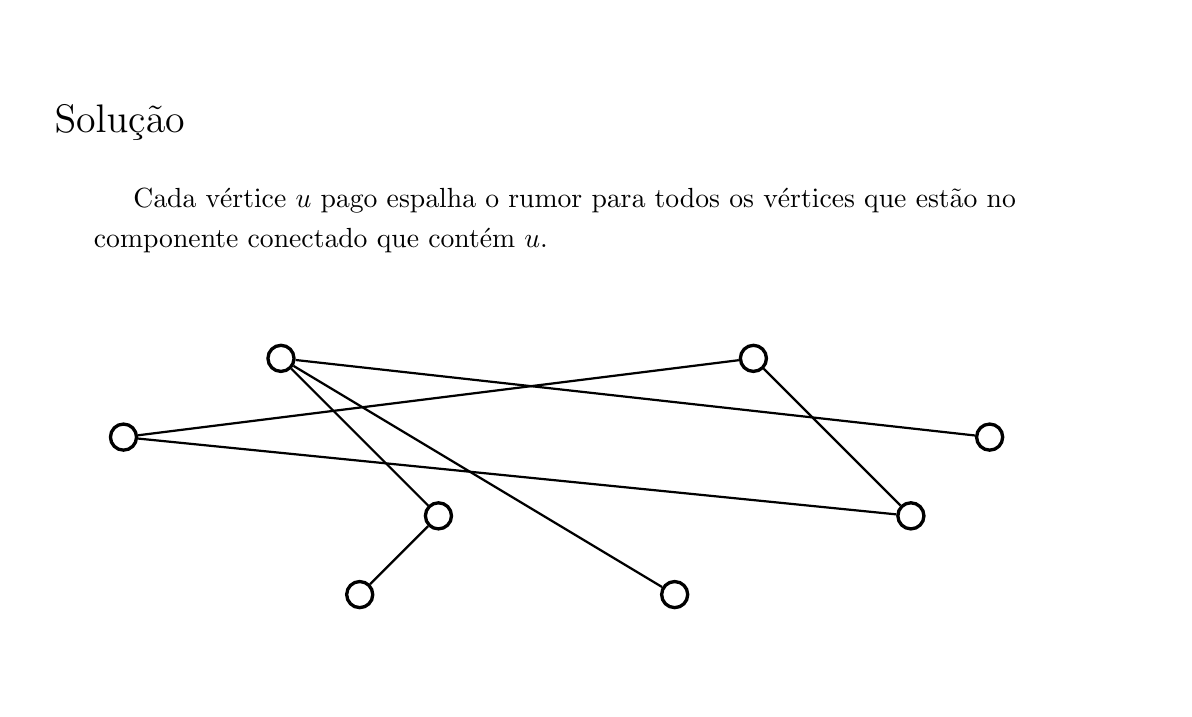
\begin{tikzpicture}
\node[draw,opacity=0] at (0, 0) {x};
\node[draw,opacity=0] at (14, 8) {x};
 \node[anchor=west] at (0, 7) { \Large \bbbold{Solução} };
 \node[anchor=west] at (1, 6) { \bbtext{Cada vértice $u$ pago espalha o rumor para todos os vértices que estão no} };
 \node[anchor=west] at (0.5, 5.5) { \bbtext{componente conectado que contém $u$.} };
 \node[draw,circle,very thick] (A) at (1, 3) { };
 \node[draw,circle,very thick] (B) at (3, 4) { };
 \node[draw,circle,very thick] (C) at (4, 1) { };
 \node[draw,circle,very thick] (D) at (5, 2) { };
 \node[draw,circle,very thick] (E) at (8, 1) { };
 \node[draw,circle,very thick] (F) at (9, 4) { };
 \node[draw,circle,very thick] (G) at (11, 2) { };
 \node[draw,circle,very thick] (H) at (12, 3) { };
 \draw[thick] (A) to (F);
 \draw[thick] (A) to (G);
 \draw[thick] (B) to (D);
 \draw[thick] (B) to (E);
 \draw[thick] (B) to (H);
 \draw[thick] (C) to (D);
 \draw[thick] (G) to (F);
\end{tikzpicture}
\end{frame}

\begin{frame}[plain,t]
\begin{tikzpicture}
\node[draw,opacity=0] at (0, 0) {x};
\node[draw,opacity=0] at (14, 8) {x};
 \node[anchor=west] at (0, 7) { \Large \bbbold{Solução} };
 \node[anchor=west] at (1, 6) { \bbtext{Cada vértice $u$ pago espalha o rumor para todos os vértices que estão no} };
 \node[anchor=west] at (0.5, 5.5) { \bbtext{componente conectado que contém $u$.} };
 \node[draw,circle,very thick] (B) at (3, 4) { };
 \node[draw,circle,very thick] (C) at (4, 1) { };
 \node[draw,circle,very thick] (D) at (5, 2) { };
 \node[draw,circle,very thick] (E) at (8, 1) { };
 \node[draw,circle,very thick] (F) at (9, 4) { };
 \node[draw,circle,very thick] (G) at (11, 2) { };
 \node[draw,circle,very thick] (H) at (12, 3) { };
 \draw[thick] (A) to (F);
 \draw[thick] (A) to (G);
 \draw[thick] (B) to (D);
 \draw[thick] (B) to (E);
 \draw[thick] (B) to (H);
 \draw[thick] (C) to (D);
 \draw[thick] (G) to (F);
 \node[draw,circle,very thick,color=BBCyan] (A) at (1, 3) { };
\end{tikzpicture}
\end{frame}

\begin{frame}[plain,t]
\begin{tikzpicture}
\node[draw,opacity=0] at (0, 0) {x};
\node[draw,opacity=0] at (14, 8) {x};
 \node[anchor=west] at (0, 7) { \Large \bbbold{Solução} };
 \node[anchor=west] at (1, 6) { \bbtext{Cada vértice $u$ pago espalha o rumor para todos os vértices que estão no} };
 \node[anchor=west] at (0.5, 5.5) { \bbtext{componente conectado que contém $u$.} };
 \node[draw,circle,very thick] (B) at (3, 4) { };
 \node[draw,circle,very thick] (C) at (4, 1) { };
 \node[draw,circle,very thick] (D) at (5, 2) { };
 \node[draw,circle,very thick] (E) at (8, 1) { };
 \node[draw,circle,very thick] (G) at (11, 2) { };
 \node[draw,circle,very thick] (H) at (12, 3) { };
 \draw[thick] (A) to (G);
 \draw[thick] (B) to (D);
 \draw[thick] (B) to (E);
 \draw[thick] (B) to (H);
 \draw[thick] (C) to (D);
 \draw[thick] (G) to (F);
 \node[draw,circle,very thick,color=BBCyan] (A) at (1, 3) { };
 \node[fill,circle,color=BBCyan] (F) at (9, 4) { };
 \node[draw,circle,very thick] (F) at (9, 4) { };
 \draw[-latex,very thick] (A) to (F);
\end{tikzpicture}
\end{frame}

\begin{frame}[plain,t]
\begin{tikzpicture}
\node[draw,opacity=0] at (0, 0) {x};
\node[draw,opacity=0] at (14, 8) {x};
 \node[anchor=west] at (0, 7) { \Large \bbbold{Solução} };
 \node[anchor=west] at (1, 6) { \bbtext{Cada vértice $u$ pago espalha o rumor para todos os vértices que estão no} };
 \node[anchor=west] at (0.5, 5.5) { \bbtext{componente conectado que contém $u$.} };
 \node[draw,circle,very thick] (B) at (3, 4) { };
 \node[draw,circle,very thick] (C) at (4, 1) { };
 \node[draw,circle,very thick] (D) at (5, 2) { };
 \node[draw,circle,very thick] (E) at (8, 1) { };
 \node[draw,circle,very thick] (H) at (12, 3) { };
 \draw[thick] (A) to (G);
 \draw[thick] (B) to (D);
 \draw[thick] (B) to (E);
 \draw[thick] (B) to (H);
 \draw[thick] (C) to (D);
 \node[draw,circle,very thick,color=BBCyan] (A) at (1, 3) { };
 \node[fill,circle,color=BBCyan] (F) at (9, 4) { };
 \node[draw,circle,very thick] (F) at (9, 4) { };
 \draw[-latex,very thick] (A) to (F);
 \node[fill,circle,color=BBCyan] (G) at (11, 2) { };
 \node[draw,circle,very thick] (G) at (11, 2) { };
 \draw[-latex,very thick] (F) to (G);
\end{tikzpicture}
\end{frame}

\begin{frame}[plain,t]
\begin{tikzpicture}
\node[draw,opacity=0] at (0, 0) {x};
\node[draw,opacity=0] at (14, 8) {x};
 \node[anchor=west] at (0, 7) { \Large \bbbold{Solução} };
 \node[anchor=west] at (1, 6) { \bbtext{Cada vértice $u$ pago espalha o rumor para todos os vértices que estão no} };
 \node[anchor=west] at (0.5, 5.5) { \bbtext{componente conectado que contém $u$.} };
 \node[draw,circle,very thick] (C) at (4, 1) { };
 \node[draw,circle,very thick] (D) at (5, 2) { };
 \node[draw,circle,very thick] (E) at (8, 1) { };
 \node[draw,circle,very thick] (H) at (12, 3) { };
 \draw[thick] (A) to (G);
 \draw[thick] (B) to (D);
 \draw[thick] (B) to (E);
 \draw[thick] (B) to (H);
 \draw[thick] (C) to (D);
 \node[draw,circle,very thick,color=BBCyan] (A) at (1, 3) { };
 \node[fill,circle,color=BBCyan] (F) at (9, 4) { };
 \node[draw,circle,very thick] (F) at (9, 4) { };
 \draw[-latex,very thick] (A) to (F);
 \node[fill,circle,color=BBCyan] (G) at (11, 2) { };
 \node[draw,circle,very thick] (G) at (11, 2) { };
 \draw[-latex,very thick] (F) to (G);
 \node[draw,circle,very thick,color=BBRed] (B) at (3, 4) { };
\end{tikzpicture}
\end{frame}

\begin{frame}[plain,t]
\begin{tikzpicture}
\node[draw,opacity=0] at (0, 0) {x};
\node[draw,opacity=0] at (14, 8) {x};
 \node[anchor=west] at (0, 7) { \Large \bbbold{Solução} };
 \node[anchor=west] at (1, 6) { \bbtext{Cada vértice $u$ pago espalha o rumor para todos os vértices que estão no} };
 \node[anchor=west] at (0.5, 5.5) { \bbtext{componente conectado que contém $u$.} };
 \node[draw,circle,very thick] (C) at (4, 1) { };
 \node[draw,circle,very thick] (E) at (8, 1) { };
 \node[draw,circle,very thick] (H) at (12, 3) { };
 \draw[thick] (A) to (G);
 \draw[thick] (B) to (E);
 \draw[thick] (B) to (H);
 \draw[thick] (C) to (D);
 \node[draw,circle,very thick,color=BBCyan] (A) at (1, 3) { };
 \node[fill,circle,color=BBCyan] (F) at (9, 4) { };
 \node[draw,circle,very thick] (F) at (9, 4) { };
 \draw[-latex,very thick] (A) to (F);
 \node[fill,circle,color=BBCyan] (G) at (11, 2) { };
 \node[draw,circle,very thick] (G) at (11, 2) { };
 \draw[-latex,very thick] (F) to (G);
 \node[draw,circle,very thick,color=BBRed] (B) at (3, 4) { };
 \node[fill,circle,color=BBRed] (D) at (5, 2) { };
 \node[draw,circle,very thick] (D) at (5, 2) { };
 \draw[-latex,very thick] (B) to (D);
\end{tikzpicture}
\end{frame}

\begin{frame}[plain,t]
\begin{tikzpicture}
\node[draw,opacity=0] at (0, 0) {x};
\node[draw,opacity=0] at (14, 8) {x};
 \node[anchor=west] at (0, 7) { \Large \bbbold{Solução} };
 \node[anchor=west] at (1, 6) { \bbtext{Cada vértice $u$ pago espalha o rumor para todos os vértices que estão no} };
 \node[anchor=west] at (0.5, 5.5) { \bbtext{componente conectado que contém $u$.} };
 \node[draw,circle,very thick] (E) at (8, 1) { };
 \node[draw,circle,very thick] (H) at (12, 3) { };
 \draw[thick] (A) to (G);
 \draw[thick] (B) to (E);
 \draw[thick] (B) to (H);
 \node[draw,circle,very thick,color=BBCyan] (A) at (1, 3) { };
 \node[fill,circle,color=BBCyan] (F) at (9, 4) { };
 \node[draw,circle,very thick] (F) at (9, 4) { };
 \draw[-latex,very thick] (A) to (F);
 \node[fill,circle,color=BBCyan] (G) at (11, 2) { };
 \node[draw,circle,very thick] (G) at (11, 2) { };
 \draw[-latex,very thick] (F) to (G);
 \node[draw,circle,very thick,color=BBRed] (B) at (3, 4) { };
 \node[fill,circle,color=BBRed] (D) at (5, 2) { };
 \node[draw,circle,very thick] (D) at (5, 2) { };
 \draw[-latex,very thick] (B) to (D);
 \node[fill,circle,color=BBRed] (C) at (4, 1) { };
 \node[draw,circle,very thick] (C) at (4, 1) { };
 \draw[latex-,very thick] (C) to (D);
\end{tikzpicture}
\end{frame}

\begin{frame}[plain,t]
\begin{tikzpicture}
\node[draw,opacity=0] at (0, 0) {x};
\node[draw,opacity=0] at (14, 8) {x};
 \node[anchor=west] at (0, 7) { \Large \bbbold{Solução} };
 \node[anchor=west] at (1, 6) { \bbtext{Cada vértice $u$ pago espalha o rumor para todos os vértices que estão no} };
 \node[anchor=west] at (0.5, 5.5) { \bbtext{componente conectado que contém $u$.} };
 \node[draw,circle,very thick] (H) at (12, 3) { };
 \draw[thick] (A) to (G);
 \draw[thick] (B) to (H);
 \node[draw,circle,very thick,color=BBCyan] (A) at (1, 3) { };
 \node[fill,circle,color=BBCyan] (F) at (9, 4) { };
 \node[draw,circle,very thick] (F) at (9, 4) { };
 \draw[-latex,very thick] (A) to (F);
 \node[fill,circle,color=BBCyan] (G) at (11, 2) { };
 \node[draw,circle,very thick] (G) at (11, 2) { };
 \draw[-latex,very thick] (F) to (G);
 \node[draw,circle,very thick,color=BBRed] (B) at (3, 4) { };
 \node[fill,circle,color=BBRed] (D) at (5, 2) { };
 \node[draw,circle,very thick] (D) at (5, 2) { };
 \draw[-latex,very thick] (B) to (D);
 \node[fill,circle,color=BBRed] (C) at (4, 1) { };
 \node[draw,circle,very thick] (C) at (4, 1) { };
 \draw[latex-,very thick] (C) to (D);
 \node[fill,circle,color=BBRed] (E) at (8, 1) { };
 \node[draw,circle,very thick] (E) at (8, 1) { };
 \draw[-latex,very thick] (B) to (E);
\end{tikzpicture}
\end{frame}

\begin{frame}[plain,t]
\begin{tikzpicture}
\node[draw,opacity=0] at (0, 0) {x};
\node[draw,opacity=0] at (14, 8) {x};
 \node[anchor=west] at (0, 7) { \Large \bbbold{Solução} };
 \node[anchor=west] at (1, 6) { \bbtext{Cada vértice $u$ pago espalha o rumor para todos os vértices que estão no} };
 \node[anchor=west] at (0.5, 5.5) { \bbtext{componente conectado que contém $u$.} };
 \draw[thick] (A) to (G);
 \node[draw,circle,very thick,color=BBCyan] (A) at (1, 3) { };
 \node[fill,circle,color=BBCyan] (F) at (9, 4) { };
 \node[draw,circle,very thick] (F) at (9, 4) { };
 \draw[-latex,very thick] (A) to (F);
 \node[fill,circle,color=BBCyan] (G) at (11, 2) { };
 \node[draw,circle,very thick] (G) at (11, 2) { };
 \draw[-latex,very thick] (F) to (G);
 \node[draw,circle,very thick,color=BBRed] (B) at (3, 4) { };
 \node[fill,circle,color=BBRed] (D) at (5, 2) { };
 \node[draw,circle,very thick] (D) at (5, 2) { };
 \draw[-latex,very thick] (B) to (D);
 \node[fill,circle,color=BBRed] (C) at (4, 1) { };
 \node[draw,circle,very thick] (C) at (4, 1) { };
 \draw[latex-,very thick] (C) to (D);
 \node[fill,circle,color=BBRed] (E) at (8, 1) { };
 \node[draw,circle,very thick] (E) at (8, 1) { };
 \draw[-latex,very thick] (B) to (E);
 \node[fill,circle,color=BBRed] (H) at (12, 3) { };
 \node[draw,circle,very thick] (H) at (12, 3) { };
 \draw[-latex,very thick] (B) to (H);
\end{tikzpicture}
\end{frame}

\begin{frame}[plain,t]
\begin{tikzpicture}
\node[draw,opacity=0] at (0, 0) {x};
\node[draw,opacity=0] at (14, 8) {x};
 \node[anchor=west] at (0, 7) { \Large \bbbold{Solução} };
 \draw[thick] (A) to (G);
 \node[draw,circle,very thick,color=BBCyan] (A) at (1, 3) { };
 \node[fill,circle,color=BBCyan] (F) at (9, 4) { };
 \node[draw,circle,very thick] (F) at (9, 4) { };
 \draw[-latex,very thick] (A) to (F);
 \node[fill,circle,color=BBCyan] (G) at (11, 2) { };
 \node[draw,circle,very thick] (G) at (11, 2) { };
 \draw[-latex,very thick] (F) to (G);
 \node[draw,circle,very thick,color=BBRed] (B) at (3, 4) { };
 \node[fill,circle,color=BBRed] (D) at (5, 2) { };
 \node[draw,circle,very thick] (D) at (5, 2) { };
 \draw[-latex,very thick] (B) to (D);
 \node[fill,circle,color=BBRed] (C) at (4, 1) { };
 \node[draw,circle,very thick] (C) at (4, 1) { };
 \draw[latex-,very thick] (C) to (D);
 \node[fill,circle,color=BBRed] (E) at (8, 1) { };
 \node[draw,circle,very thick] (E) at (8, 1) { };
 \draw[-latex,very thick] (B) to (E);
 \node[fill,circle,color=BBRed] (H) at (12, 3) { };
 \node[draw,circle,very thick] (H) at (12, 3) { };
 \draw[-latex,very thick] (B) to (H);
 \node[anchor=west] at (1, 6) { \bbtext{Logo, basta pagar o vértice de menor custo em cada componente conectado.} };
\end{tikzpicture}
\end{frame}

\begin{frame}[plain,t]
 \inputsnippet{cpp}{11}{21}{codes/893C.cpp}
\end{frame}

\begin{frame}[plain,t]
 \inputsnippet{cpp}{23}{40}{codes/893C.cpp}
\end{frame}

\end{document}
